\chapter{REQUIREMENT ANALYSIS}

% \section{Introduction}
% 	This project aims to empower users to make informed fashion choices and enhance their online shopping experience by seamlessly integrating AI algorithms for clothing recommendations and virtual try-on technology. In an era where online shopping dominates, our system seeks to empower consumers with a personalized shopping experience.

% 	\subsection{Purpose}
% 		The main goals of this project are to elevate the online shopping experience of customers by using AI to provide them with personalized clothing recommendations and AR virtual try-on, to reduce uncertainty associated with online purchases and by extension, reduce item return rates.

% 	\subsection{Project Scope}
% 		The project has the following scope:

% 		\begin{enumerate}
% 			\item \textbf{Fashion embedding:} Fashion embedding is a pivotal component, serving as the foundation for further tasks.
% 				\begin{enumerate}
% 					\item \textit{High-dimensional representation:} The project will transform clothing items into high-dimensional representations in a latent space. Each item will be associated with a vector that encodes its unique features and attributes.
% 					\item \textit{Recommendation:} These fashion embeddings will play a fundamental role in the recommendation system. They will enable the model to identify similarities and compatibilities between items, effectively suggesting products based on user preferences and past interactions. Recommendations will be made by locating items with embeddings closely aligned with the user's preferences.
% 					\item \textit{Retrieval:} The fashion embeddings will facilitate efficient and accurate retrieval of items. Users will be able to search for specific items or styles by querying the embedded space, and the system will quickly locate relevant matches.
% 					\item \textit{Semantic understanding:} The high-dimensional embeddings will capture the semantic meaning and context of fashion items, going beyond visual features. This means that items with similar semantic attributes can be effectively grouped together.
% 				\end{enumerate}
% 			\item \textbf{Feature extractor:} Use deep learning to train a feature extractor which can segment parts of the upper body to provide user features for attribute-based recommendations, and to detect rendering regions for virtual try-on.
% 			\item \textbf{AI-based recommender:} Design and deploy a recommendation system that utilizes collaborative and content-based filtering to generate personalized clothing recommendations.
% 				\begin{enumerate}
% 					\item \textit{Train with body dimensions:} Fine-tune system to take into account various body dimensions, such as waist size, chest measurements, and height.
% 					\item \textit{Recommendations tailored to physique:} Provide clothing recommendations suitable for lean to average body sizes of average body length. Offer suggestions that are not only stylish but also appropriately sized.
% 				\end{enumerate}
% 			\item \textbf{AR virtual try-on:} Develop an AR-based virtual try-on system that allows users to visualize and interact with clothing items in real-time.
% 				\begin{enumerate}
% 					\item \textit{Dynamic and responsive:} Design a dynamic and responsive system with which users can try on multiple clothing items and evaluate them one by one.
% 					\item \textit{Device compatibility:} Ensure system is compatible with a range of devices, including smartphones, tablets, and desktops, making it accessible to a wide user base.
% 					\item \textit{User-Friendly Interface:} Design an user interface which is intuitive and user-friendly, ensuring that users can easily navigate and interact with the virtual try-on features.
% 				\end{enumerate}
% 		\end{enumerate}

% \section{Overall Description}
% 	\subsection{Product Perspective}
% 		Our project operates within the context of the broader e-commerce and fashion retail landscape. It aims to integrate with e-commerce platforms, acting as an enhancement to the shopping experience. This system augments traditional online shopping by providing intelligent clothing recommendations and a virtual try-on feature. It does not replace or compete with e-commerce platforms but complements their functionality, aiming to boost user engagement and sales. By focusing on user experience, the project seeks to align with the goals of e-commerce businesses, creating a symbiotic relationship that benefits both consumers and retailers.
	
% 	\subsection{Product Functions}
% 		The project has the following product functions:

% 		\begin{enumerate}
% 			\item \textbf{User profiles:} Users can create accounts and profiles, providing personal information, style preferences, and body measurements. Profiles are used to tailor clothing recommendations to individual user preferences.
% 			\item \textbf{Clothing recommender:} Utilizes AI algorithms to analyze user data and style preferences and generates personalized clothing recommendations based on the user's profile.
% 			\item \textbf{Search and browsing:} Allows users to search for clothing items or browse through a selection of recommended items. Filters, sorting options, and search functionality enhance the browsing experience.
% 			\item \textbf{Virtual try-On:} Employs augmented reality (AR) technology to enable users to virtually try on clothing items. Overlays selected garments on the user's real-time image or avatar to visualize fit and appearance. Supports various angles and poses to ensure an accurate representation.
% 			\item \textbf{User feedback:} Allows users to rate and review purchased items. Collects valuable feedback to improve the recommendation system.
% 		\end{enumerate}

% 		\begin{figure}
% 			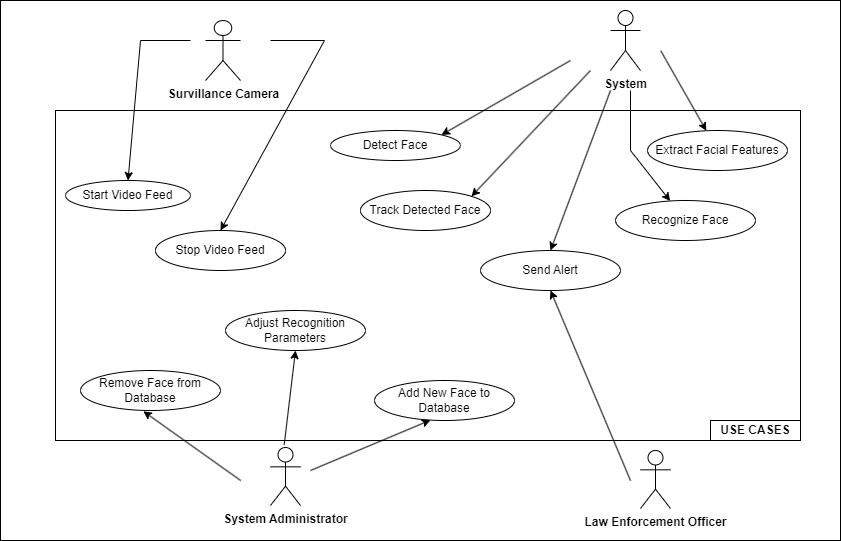
\includegraphics[width=\textwidth]{components/images/use-case.png}
% 			\caption{Use-case diagram}
% 			\label{fig:use-case}
% 		\end{figure}

% 	\subsection{User Classes and Characteristics}
% 		The project has the following user classes: 

% 		\begin{enumerate}
% 			\item \textbf{Online shoppers:}
% 				\begin{itemize}
% 					\item \textit{Characteristics:} Shoppers are the primary end-users of the system. They have varying fashion preferences and seek clothing recommendations that align with their personal style and body type. Shoppers may have different levels of technological proficiency, from tech-savvy individuals to those with limited technology experience.
% 					\item \textit{Usage:} Shoppers use the system to search for clothing items, receive personalized recommendations, and virtually try on garments. They provide feedback and ratings to refine future recommendations.
% 				\end{itemize}
% 			\item \textbf{Retailers and fashion brands:}
% 				\begin{itemize}
% 					\item \textit{Characteristics:} Retailers and fashion brands represent business partners or clients who wish to integrate the recommendation and virtual try-on system into their e-commerce platforms. They possess in-depth knowledge of their product catalogs and seek to improve customer engagement and sales.
% 					\item \textit{Usage:} Retailers and fashion brands collaborate with the development team to integrate the system into their online stores. They may provide fashion catalogs, branding assets, and participate in system customization.
% 				\end{itemize}
% 			\item \textbf{Fashion designers and stylists:}
% 				\begin{itemize}
% 					\item \textit{Characteristics:} Fashion designers and stylists may collaborate with the system to showcase their clothing collections or styling expertise. They are experts in fashion trends, design, and styling.
% 					\item \textit{Usage:} Designers and stylists work with retailers to curate clothing collections and styles for the system. They may also provide fashion tips, styling advice, or content to enrich the user experience.
% 				\end{itemize}
% 			\item \textbf{Data analysts and AI specialists:}
% 				\begin{itemize}
% 					\item \textit{Characteristics:} Data analysts and AI specialists are responsible for fine-tuning the recommendation algorithms and ensuring the system's AI components work optimally. They possess expertise in data analysis and machine learning.
% 					\item \textit{Usage:} Data analysts and AI specialists continuously improve recommendation algorithms, analyze user data for patterns, and adapt the system to evolving fashion trends and customer preferences.
% 				\end{itemize}
% 		\end{enumerate}

% \section{Specific Requirements}
% 	\subsection{Operating Environment}
% 		The operating environment of our project is as follows:

% 		\begin{enumerate}
% 			\item \textbf{Software requirements:}
% 				\begin{itemize}
% 					\item \textit{Operating system:} The target end-user operating system may be any of the following platforms which support the ONNX Runtime \cite{onnxruntimeCompatibility}:
% 						\begin{itemize}
% 							\item Windows 10 1709+
% 							\item Linux distributions supported by .NET Core
% 							\item Mac 10.14+ (Mojave)
% 							\item Android 28+ (v9 ``Pie")
% 							\item iOS 12+
% 						\end{itemize}
% 					\item \textit{Web browsers:} It should be accessible through popular web browsers like Google Chrome, Mozilla Firefox, Safari, and Microsoft Edge for web-based interfaces.
% 					\item \textit{AR framework:} A robust AR framework such as AR.js for web-based AR experiences, should be integrated.
% 					\item \textit{Database management:} The project requires a database management system for user profiles, clothing item information, and preference data. Document-based NoSQL options like Apache Cassandra can be considered.
% 					\item \textit{Programming languages and libraries:} Development will involve languages like Python and JavaScript, and frameworks like PyTorch and Huggingface Transformers and Optimum for machine learning tasks.
% 					\item \textit{Machine learning inference:} A cross-platform machine learning runtime like ONNX Runtime which supports the ONNX format, an open standard for machine learning interoperability.
% 					\item \textit{Web development stack:} For web-based interfaces, a stack including HTML, CSS, JavaScript, and backend frameworks like Node.js and Express will be employed.
% 				\end{itemize}
% 			\item \textbf{Hardware requirements:}
% 			\begin{itemize}
% 				\item \textit{User devices:} The project is intended to work on a range of user devices like smartphones, tablets, laptops, and desktop computers.
% 				\item \textit{Cameras and sensors:} Devices should have integrated or attachable cameras and sensors capable of capturing user images and surroundings for the virtual try-on feature.
% 				\item \textit{CPU:} Any modern multi-core processor with a clock speed of at least 2.5 GHz.
% 				\item \textit{GPU:}
% 					\begin{itemize}
% 						\item Training requirement: A video-card with minimum 8GB VRAM for deep learning tasks.
% 						\item End-user inference requirement: Any GPU which supports Vulkan APIs.
% 					\end{itemize}
% 				\item \textit{Internet connectivity:} A stable internet connection is essential for real-time communication with the server, image processing, and rendering of AR elements.
% 			\end{itemize}
% 		\end{enumerate}
	
% 	\subsection{Design Philosophies}
% 		\begin{enumerate}
% 			\item \textbf{User-centric design:} Our design philosophy places the user at the center of the system. We prioritize creating an intuitive and seamless user experience that accommodates users of various demographics and technological backgrounds. User feedback will continuously inform design improvements.
% 			\item \textbf{Personalization:} The system will employ machine learning algorithms to create a highly personalized experience. User preferences and feedback will be used to tailor clothing recommendations and enhance the virtual try-on experience.
% 			\item \textbf{Scalability:} The design will be modular and scalable to accommodate a growing user base and evolving technological trends. This approach allows for easy integration of new features and accommodates increased usage loads.
% 			\item \textbf{Security and privacy:} Security and privacy will be fundamental to the design, with strong encryption protocols for data protection. Users' personal information and imagery will be handled with the utmost care, and adherence to data protection regulations is a priority.
% 		\end{enumerate}

% 	\subsection{Implementation Philosophies}
% 		\begin{enumerate}
% 			\item \textbf{State-of-the-Art AI:} Implementation will involve integrating state-of-the-art machine learning and computer vision techniques to ensure accurate clothing recommendations and realistic virtual try-on experiences. We will employ libraries and frameworks with active development and community support.
% 			\item \textbf{Cross-platform compatibility:} The system will be developed with cross platform compatibility in mind. Web interfaces will be developed to ensure that users can access and utilize the system seamlessly on various devices.
% 			\item \textbf{Continuous testing and iteration:} Agile development methodologies will be used to enable continuous testing, feedback, and iteration. This approach allows us to respond to user needs, refine algorithms, and enhance system performance throughout development.
% 		\end{enumerate}

% 	\subsection{Constraints}
% 		\begin{enumerate}
% 			\item \textbf{Data Privacy and Compliance:} The project must adhere to strict data privacy regulations. This imposes constraints on how user data is collected, stored, and utilized.
% 			\item \textbf{Resource Limitations:} The project will operate within resource constraints, including budget and available hardware resources, which may affect the system's scalability and performance.
% 			\item \textbf{Technological Compatibility:} The system must work across a wide range of devices and platforms, which presents constraints related to compatibility and performance optimization.
% 			\item \textbf{User Connectivity:} User experience may be affected by the quality of the user's internet connection, especially when utilizing the augmented reality feature. Ensuring a functional experience even in low-bandwidth situations is a constraint.
% 		\end{enumerate}

% \section{External Interface Requirements}
% 	\subsection{User Interfaces}
% 		The primary user interface will be web-based and accessible via standard web browsers. It should be compatible with popular web browsers, including but not limited to Google Chrome, Mozilla Firefox, Microsoft Edge, and Safari. The user interface should be responsive, adapting to various screen sizes, including desktops, tablets, and mobile devices.

% 		The virtual try-on interface relies on AR and should be compatible with most devices. It must support features such as real-time clothing overlay and interactive controls for users to try on clothing items seamlessly.
	
% 	\subsection{Hardware Interfaces}
% 		The virtual try-on feature requires the use of cameras and sensors. Our system should interface with these devices to capture images and detect user movements for an immersive AR experience. These interfaces should be compatible with a range of devices.

% 	\subsection{Software Interfaces}
% 		\subsubsection{Clothing Recommendation Interface}
% 			The system will interface with a clothing recommendation algorithm to leverage advanced recommendation algorithms for personalized clothing suggestions.

% 			Requirements:
% 			\begin{enumerate}
% 				\item The system should send user profile and preferences data to the recommendation algorithm.
% 				\item The algorithm should return a list of recommended clothing items.
% 				\item The interface should allow for updates to the recommendation algorithm without affecting core system functionality.
% 			\end{enumerate}
		
% 		\subsubsection{AR Virtual Try-On Interface}
% 			The system will interface with an AR module for virtual clothing try-on to enable users to visualize clothing items on themselves in real-time.

% 			Requirements:
% 			\begin{enumerate}
% 				\item The AR module must support 3D model rendering of clothing items on user images.
% 				\item It should provide accurate real-time visualization.
% 				\item The system should send data about selected clothing items to the AR module for rendering.
% 				\item The AR module should return rendered images or video streams of users with clothing items superimposed.
% 			\end{enumerate}

% 		\subsubsection{User Profile and Preferences Data Interface}
% 			The system will interact with user profile and preferences data to gather information about user preferences and characteristics for clothing recommendations.

% 			Requirements:
% 			\begin{enumerate}
% 				\item The system must allow users to create and update their profiles.
% 				\item It should securely store and retrieve user data.
% 				\item The interface must be compliant with data protection regulations.
% 			\end{enumerate}

% \section{Other Nonfunctional Requirements}
% 	\subsection{Performance Requirements}
% 		The system should be able to read and understand the human body and be able to parse the areas of interests, generate outfit accordingly and finally, render the subject in real-time through augmented reality.
		
% 		\subsubsection{Resource utilization}
% 			For the system to be compatible with majority devices including low powered mobiles and tablets, the resource utilization should be kept to minimum without affecting the quality of output.

% 		\subsubsection{Feedback duration}
% 			As expected of the try-on systems, the system should be able to provide feedback on the subject in real-time. Processing time should be kept as low as possible for better experience for user.

% 		\subsubsection{Feedback quality}
% 			The system should generate personalized outfit and the subject should be able to judge the proposed style and size on itself. The process should be both convenient and rewarding for the user.
		
% 	\subsection{Safety and Security Requirements}
% 		\begin{enumerate}
% 			\item \textbf{Privacy compliance:} The user shouldn't be concerned about disclosure of his/her features to open userbase. The system should only parse the regions of interest for building the metrics of generation and should not intent to perform any malicious operations.
% 			\item \textbf{Ethics:} The system should not delve into inappropriate outfit generation and should take into account of user's modesty. The system shouldn't be biased towards certain age groups, races or color.
% 			\item \textbf{Compliances:} The system should adhere to rules and compliances stated by the authorities and stakeholders and should limit it's working domain to that specified be the compliances.
% 		\end{enumerate}
	
% 	\subsection{Acceptance Criteria}
% 		Give the scenario where the user has selected certain clothes according to their preferences and is expecting the system to generate the outfit on their body so that they can judge the style and the overall look of the outfit, the user lets the camera record their body. Both the subject body features and generated recommendations are input for the system.

% 		When the user selects generate outfit option after selection of styles recommended or chosen by himself/herself. The system segments the features from the subject and tries to wrap the outfit around them. If the system is well trained on personalized recommendation and virtual try-on, the system successfully generates the outfit personalized to the subject and provides the rendered view in augmented reality.

% 	\subsection{Software Quality Attributes}
% 		\begin{enumerate}
% 			\item \textbf{Reliability:} The system should be dependable, providing accurate clothing recommendations and ensuring that the virtual try-on feature functions consistently without errors or crashes.
% 			\item \textbf{Usability:} User interfaces should be intuitive and user-friendly, making it easy for customers to navigate the system and obtain clothing suggestions effortlessly.
% 			\item \textbf{Maintainability:} The codebase should be well-organized, documented, and structured to facilitate updates, enhancements, and bug fixes.
% 			\item \textbf{Flexibility:} The system should adapt to changes in user preferences, allowing for the integration of new fashion items and the modification of recommendation algorithms.
% 			\item \textbf{Robustness:} The system should be able to handle unexpected inputs or situations without crashing or providing inaccurate results.
% 		\end{enumerate}

% \section{Future Scope}
% 	The project opens up the following future developments:

% 	\begin{enumerate}
% 		\item Inclusion of more body types.
% 		\item Extended clothing categories and varieties.
% 		\item Multi-modal integration such as voice-activated commands and gesture-based interactions for enhanced virtual try-ons.
% 		\item Integration of social media elements.
% 		\item Integration with wearable technology.
% 		\item Fashion trend analysis and prediction to aide recommendations.
% 	\end{enumerate}

\section{Introduction}
    In the rapidly advancing domain of law enforcement, the emergence of real-time face recognition is a pivotal tool for enhancing security, optimizing response times, and bolstering crime prevention and investigative capabilities. However, the practical deployment of such real-time facial recognition systems is rife with complexities, especially when applied to the dynamic and often unpredictable scenarios encountered in law enforcement. Challenges such as occlusions, dynamic backgrounds, and the inherent intricacies of tracking multiple individuals in crowded settings underscore the need for robust, efficient, and reliable systems. This section is geared towards detailing the prerequisites, desired functionalities, and specifications for the development of an advanced real-time face recognition system tailored to meet the unique needs and challenges of law enforcement.
    
    \subsection{Purpose}
    Develop a real-time face recognition system tailored specifically for law enforcement. This system is designed to enhance security measures, facilitate faster responses, and offer more effective crime prevention and investigation by swiftly and accurately identifying individuals in the field. It aims to navigate and address the inherent challenges in real-world law enforcement scenarios, such as facial occlusions due to masks or sunglasses, recognition in crowded settings, and varying backgrounds. The system seeks to optimize the process of face detection, tracking, and recognition, ensuring it meets the unique demands and high stakes of law enforcement scenarios.
    
    \subsection{Project Scope}
    This project's scope includes creating an real time face recognition system that can match the detected face with a database in real-time, allowing for swift identification. It also consists of a secure and scalable database to store facial data. This database can be updated as required, allowing for additions, modifications, or deletions.    Providing thorough documentation to help users deploy and utilize the system efficiently is another aspect of the scope. The project's scope is set to ensure that the system is not just accurate but also practical for the high-stakes, dynamic environments in which law enforcement operates.


\section{Overall Description}
    \subsection{Product Perspective}
        It operates within a broader system perspective, integrating seamlessly with existing law enforcement surveillance infrastructure. This system serves as a modular component, capable of functioning both independently and as an integral part of the surveillance ecosystem. Its main functions encompass face detection, tracking, real-time recognition, and alert generation. The face recognition system complements the surveillance network by enhancing security and investigative capabilities, and it offers a vital tool that promises to revolutionize law enforcement operations. Its versatility in either standalone operation or integration into existing systems ensures flexibility and adaptability to various law enforcement scenarios, positioning it as a valuable asset in the realm of real-time face recognition for law enforcement purposes.
    
    \subsection{Product Functions}
        The product, a real-time face recognition system for law enforcement, has several core functions. Some of the functions are:
        \begin{itemize}
            \item \textbf{Face Detection:} The system can scan and identify human faces from various sources such as images, videos, and live surveillance feeds. This function can handle multiple faces simultaneously even in crowded scenes and identify them in varying lighting conditions and angles.
            \item \textbf{Face Tracking:} After detecting faces, the system has the capability to track individual faces across a sequence of frames or video streams. It maintains continuity, even if the face undergoes temporary occlusions, movements, or changes in expression.
            \item \textbf{Real-time Face Recognition:} By comparing detected faces against a database of known individuals, the system can swiftly and accurately identify persons of interest. This function is invaluable in law enforcement settings, where the prompt identification of a suspect or missing person can be crucial.
            \item \textbf{Alert Generation:} When the system identifies a match or encounters a predefined scenario (e.g., an individual from a watchlist appearing in a restricted area), it generates real-time alerts. These notifications can be forwarded to law enforcement officers or other relevant personnel for immediate action.
            \item \textbf{Integration with Existing Surveillance Systems:} The product seamlessly integrates with current surveillance infrastructure, making it a plug-and-play solution that enhances the capabilities of existing systems.
        \end{itemize}
    
    \subsection{User Classes and Characteristics}
        The various user classes interacts with the system differently and has unique needs, which should be considered during the system design and development phase to ensure a comprehensive and efficient product. 
        \begin{enumerate}
            \item \textbf{Law Enforcement Officers (On-field):}
                \begin{itemize}
                    \item Typically operate in the field and require real-time data.
                    \item Need simple, intuitive interfaces due to the critical nature of their work.
                    \item May not have extensive technical expertise but are trained for basic operations.
                    \item Rely heavily on the accuracy and timeliness of the face recognition system.
                    \item Require alerts and notifications for immediate actions.     
                \end{itemize}
            \item \textbf{Surveillance Operators:}
                \begin{itemize}
                    \item Usually stationed in control rooms monitoring multiple feeds.
                    \item Need advanced filtering options to focus on specific camera feeds or regions.
                    \item Have a moderate level of technical expertise.
                    \item Need tools for playback, zoom, and other video controls.
                    \item Prioritize system stability and seamless integration with existing surveillance infrastructure.    
                \end{itemize}
            \item \textbf{Forensics and Investigation Teams:}
                \begin{itemize}
                    \item Use the system for post-incident analysis rather than real-time monitoring.
                    \item Require advanced search functionalities, including partial face recognition, timestamp filtering, and location-based searching.
                    \item Need capabilities for evidence documentation, including exporting clips, snapshots, or recognition reports.
                    \item Highly trained and have a mix of technical and investigative expertise. 
                \end{itemize}
            \item \textbf{System Administrators:}
                \begin{itemize}
                    \item Responsible for the maintenance, updates, and overall health of the face recognition system.
                    \item Need advanced administrative controls, including user management, system diagnostics, and backup utilities.
                    \item Highly technical and have a deep understanding of the system's infrastructure and its integration points.   
                \end{itemize}
            
        \end{enumerate}
    
    \subsection{Operating Environment}
        The system will operate on Windows-based systems primarily. It will require a sufficiently powerful CPU and GPU to run efficiently. Detailed description is provided below:
        \begin{enumerate}
            \item \textbf{Hardware Platform:}
                The software is designed to operate on a variety of hardware platforms, but it performs optimally with the following specifications:
                \begin{itemize}
                    \item \textit{CPU:} A modern multi-core processor (e.g., Intel Core i5 or AMD Ryzen 5) with a clock speed of at least 2.5 GHz.
                    \item \textit{GPU:} Nvidia GeForce or AMD Radeon series GPUs are recommended.
                    \item \textit{RAM:} A minimum of 8 GB of RAM for efficient processing and multitasking.
                    \item \textit{Storage:} Adequate free storage space for the operating system (preferably Solid-State Drive).
                    \item \textit{Surveillance Cameras:} Integration with a wide array of camera models and types, including IP cameras, PTZ cameras, thermal imaging cameras, and body-worn cameras.
                    \item \textit{End-User Devices:} Compatible with standard workstations in control rooms, mobile devices for on-field officers, and specialized terminals for surveillance operators.
                \end{itemize}
            \item \textbf{Software Environment:}
                \begin{itemize}
                    \item \textit{Operating System:} Compatible with Windows 10 and later versions (64-bit).
                    \item \textit{Database Management:} Compatible with leading database management systems, ensuring smooth and efficient storage and retrieval of facial data, recognition logs, and system analytics.
                    \item \textit{Integration Modules:} Built-in connectors for integrating with existing surveillance software, law enforcement databases, and other critical third-party systems.                    
                \end{itemize}
            \item \textbf{Network Environment: }
                \begin{itemize}
                    \item \textit{Local Area Network (LAN):} Designed to operate efficiently within intranet environments, especially for high-bandwidth operations like streaming video feeds.
                    \item \textit{Wide Area Network (WAN):} Capable of remote operations, ideal for connecting distant locations, and enabling mobile access.
                    \item \textit{Internet:} Provides secure internet-based access for remote surveillance monitoring, administrative tasks, and system updates. Uses encrypted connections and complies with best practices for cybersecurity.
                \end{itemize}
        \end{enumerate}
        By ensuring compatibility with these hardware and software components, the system can effectively operate and provide reliable results for its users.
    
    
    \subsection{Design and Implementation Constraints}
        \begin{enumerate}
            \item \textbf{Hardware Limitations}
            The system's efficiency is directly proportional to the hardware it operates on. Advanced facial recognition algorithms, especially those leveraging deep learning, require powerful computational resources. The minimum hardware requirement needs to be strictly adhered to for optimal performance.
            \item \textbf{Data Privacy and Security}
            Given the sensitive nature of facial data, strict encryption and cybersecurity protocols must be maintained. The system must comply with prevailing data protection regulations and laws.
            \item \textbf{Network Dependence}
            The system's efficiency depends on the stability and speed of the network. Any latency or network disruptions can impede its real-time recognition capabilities.
            \item \textbf{Integration with Existing Systems}
            The design must be adaptable and modular to ensure smooth integration with various surveillance systems, databases, and third-party tools already in use by law enforcement agencies.
            \item \textbf{Software Licensing}
            Some third-party tools, libraries, or software components that the system might rely on could have licensing restrictions, which could impact the distribution, modification, or commercialization of the system.
            \item \textbf{Continuous Training}
            For the system to maintain its effectiveness, the underlying models might need periodic retraining, which would require access to fresh, labelled data. This ongoing need can be a constraint for maintaining the system's accuracy over time.
            \item  \textbf{Scalability}
            As the user base grows and more data is fed into the system, its design should allow for easy scalability without a significant overhaul.
        \end{enumerate}
    
    \subsection{User Documentation}
        Comprehensive user documentation will be provided, including installation guides, usage instructions, and troubleshooting tips. Users will also have access to a knowledge base for common issues and solutions. Some documentation that will be provided are:
        \begin{enumerate}
                \item \textbf{User Manual:}
                    \begin{itemize}
                        \item \textit{Delivery Format:} PDF and online knowledge base.
                        \item \textit{Standards:} The user manual will adhere to standard technical writing conventions, including clear instructions, diagrams, and an easy-to-navigate structure.
                    \end{itemize}
                \item \textbf{Video Tutorials:}
                    \begin{itemize}
                        \item \textit{Delivery Format:} Video files (e.g., MP4) hosted on a dedicated platform (e.g., YouTube or GitHub).
                        \item \textit{Standards:} Video tutorials will be created with professional video editing software and include voiceovers or captions for accessibility.    
                    \end{itemize}
                \item \textbf{FAQs and Troubleshooting Guide:}
                    \begin{itemize}
                        \item \textit{Delivery Format:} PDF and online knowledge base.
                        \item \textit{Standards:} FAQs and troubleshooting guides will be organized logically, with concise answers to common questions and step-by-step troubleshooting procedures. Online versions will be easily searchable.
                    \end{itemize}
                \item \textbf{Release Notes:}
                    \begin{itemize}
                        \item \textit{Delivery Format:} PDF or readme files.
                        \item \textit{Standards:}  Release notes will follow a standardized format, providing information about software updates, bug fixes, and new features. They will also include version history and known issues.
                    \end{itemize}
            \end{enumerate}
    
    \subsection{Assumptions and Dependencies}
        \subsubsection{Assumptions}
            \begin{enumerate}
                \item \textbf{User Competency:} The assumption is that users, especially law enforcement personnel, have a basic understanding of technology and can follow the provided user documentation.
                \item \textbf{Security Protocols:} The system assumes that standard security protocols are followed, and there's protection against potential cyber threats.
                \item \textbf{Quality of Training Data:} The effectiveness of the system depends on the quality of training data used to develop its decision-making algorithms. It's assumed that the required datasets for training and testing, especially those pertaining to faces, are available and have been processed ethically and legally.
                \item \textbf{Stable Internet Connection:} The system assumes a stable and high-speed internet connection for real-time processing, especially when integrating with cloud databases or accessing remote resources.
            \end{enumerate}
        \subsubsection{Dependencies}
            \begin{enumerate}
                \item \textbf{Hardware Specifications:} The project is dependent on the capabilities of the hardware on which it will be deployed. The performance of the system may vary based on CPU and GPU capabilities.
                \item \textbf{Operating System Support:} The AI agent is designed to operate on Windows systems. It relies on the stability and compatibility of the operating system.
                \item \textbf{Third-party Libraries:} The face recognition system might rely on certain third-party libraries or frameworks, especially for deep learning and image processing functionalities.
                \item \textbf{Database Systems:} The system's functionality might depend on specific database systems for storing and retrieving face data, user information, and logs.
                \item \textbf{Regulatory Compliance:} The system's operations might depend on adherence to specific regional or international standards and regulations related to data privacy, surveillance, and law enforcement.
                \item \textbf{Peripheral Devices:} The system's real-time processing might depend on specific models or versions of cameras, sensors, or other peripheral devices.
                \item \textbf{User Knowledge:} Users are assumed to have a basic understanding of the games being tested. Inexperienced or unfamiliar users may not effectively configure or use the AI agent.
                \item \textbf{Network Connectivity:} While the AI agent primarily operates locally, it may require occasional internet access for updates or data sharing. It assumes a stable network connection for such purposes.
            \end{enumerate}


\section{External Interface Requirements}
    \subsection{User Interfaces}
        \subsubsection{Components}
            \begin{enumerate}
                \item \textbf{Dashboard Interface:} A user-friendly dashboard that provides an overview of system statistics, recent matches, alerts, and ongoing operations. This will most likely be web based.
                \item \textbf{Search and Filter Interface:} Allows users to search through the database, filter results based on specific criteria, and view detailed information on identified individuals.
                \item \textbf{Alert and Notification Panel:}  Real-time alerts for matches, especially for individuals of interest.
                \item \textbf{Performance Monitoring:} Users will be able to monitor the system's performance in real-time. The interface will display key metrics such as score, completion time, and any other relevant data.
                \item \textbf{Report Generation:} Interface to generate and view various reports, such as match accuracy, system usage, or flagged individuals.
            \end{enumerate}
        \subsubsection{Standards and constraints}
            \begin{enumerate}
                \item \textbf{Error Handling:} Error messages will follow a standardized format to provide clear and informative feedback to users when they enter invalid commands or encounter issues.
                \item \textbf{Keyboard Shortcuts:} Keyboard shortcuts will be supported to streamline user interaction. For example, users can press "Ctrl+H" to access the help menu.
            \end{enumerate}
    
    \subsection{Hardware Interfaces}                
            \begin{enumerate}
                \item \textbf{GPU Interaction:} The system will be physically connected to the GPU through PCIe (Peripheral Component Interconnect Express) slots on the motherboard. It will access the GPU's memory and processing capabilities to capture frames and perform real-time image analysis. Compatibility with different GPU models and manufacturers will be ensured through standardized APIs and driver support.
                \item \textbf{Camera Integration:} Interface to connect, configure, and retrieve feeds from multiple surveillance cameras or devices.
                \item \textbf{Power Requirements:} The system may have specific power requirements, which will vary depending on the hardware components used. It should be designed to operate within the power limits of the host system to prevent overheating or hardware damage.
                \item \textbf{Peripheral Devices:} Integration points for devices like alarms, door controls, or other alert systems.
                \item \textbf{Storage Devices:} Interface to access and store data on external storage devices, be it HDDs, SSDs, or network storage.
            \end{enumerate}
    
    \subsection{Software Interfaces}
            \begin{enumerate}
                \item \textbf{Development Tools and Libraries:} The agent will utilize machine learning frameworks like TensorFlow (version 2.6) and PyTorch (version 2.X) for training and inference. It may also incorporate computer vision libraries such as OpenCV (version 4.5) for image processing. The communication with these libraries and tools will involve calling their APIs to execute machine learning models and image analysis tasks.
                \item \textbf{Database Integration:} The system will need an interface to interact with the underlying database, whether it's for retrieving stored facial data or saving new information.
                \item \textbf{APIs for Third-Party Integration:} Open APIs or integration points to connect with other law enforcement systems, such as criminal databases, incident reporting systems, or other surveillance tools.
                \item \textbf{Operating Systems:} The system will be designed to run on  Windows (Windows 10 and Windows 11).
                \item \textbf{Security Protocols:} Interfaces to integrate with security solutions like firewalls, intrusion detection systems, and encryption tools to ensure data privacy and system integrity.
            \end{enumerate}
    \subsection{Data sharing mechanism}
        Data sharing across software components will primarily be achieved through structured data formats, such as JSON or XML, for passing information between the agent and game engines, bug tracking systems, and the database.


\section{System Features}  
    \subsection{System Feature 1: Real-time Face Detection}   
        \subsubsection{Description}
            The system will scan live video feeds to detect human faces in real-time, differentiating facial structures from the background and other objects.
        \subsubsection{Functionalities}
            \begin{itemize}
                \item Detect multiple faces simultaneously in crowded scenes.
                \item Recognize occlusions like masks, sunglasses, and hats and adjust detection strategies accordingly.
                \item Offer adjustable sensitivity settings for detection accuracy.                
            \end{itemize}
    
    \subsection{System Feature 2: Face Tracking}   
        \subsubsection{Description}
            Once a face is detected, the system will continuously track its movement across multiple frames, maintaining focus even if the face is momentarily obscured or turns away.
        \subsubsection{Functionalities}
            \begin{itemize}
                \item Multi-face tracking in dense environments.
                \item Handle sudden movements or changes in face orientation.
                \item Predict movement paths for smoother tracking.
                               
            \end{itemize}

    
        \subsection{System Feature 3: Facial Feature Extraction}   
            \subsubsection{Description}
            Extract and analyse facial features to create a unique identifier for each face.
            \subsubsection{Functionalities}
                \begin{itemize}
                    \item Identify key landmarks such as eyes, nose, mouth, and jawline.
                    \item Generate a feature vector for each face that serves as its signature.
                    \item Store feature vectors in a database for comparison and recognition.                
                \end{itemize}
        
                \subsection{System Feature 4: Face Recognition}   
                \subsubsection{Description}
                Compare the extracted facial features against a database to identify the individual.
                \subsubsection{Functionalities}
                    \begin{itemize}
                        \item Low latency comparison algorithms to provide instant recognition.
                        \item Handle slight variations in appearance, such as aging or minor cosmetic changes.
                        \item Display potential matches with a confidence score.
                                    
                    \end{itemize}
    
                    \subsection{System Feature 5: Alerts and Notifications System}   
                    \subsubsection{Description}
                    Notify users in real-time when specific individuals are recognized, especially those marked of interest.
                    \subsubsection{Functionalities}
                        \begin{itemize}
                            \item Customizable alert settings based on user requirements.
                            \item Integration with external alerting systems, such as alarms or mobile notifications.
                            \item Log and archive all alerts for future reference.         
                        \end{itemize}

                        \subsection{System Feature 6: Interactive Dashboard}   
                        \subsubsection{Description}
                        A user interface providing an overview of system operations, statistics, and access to various functionalities.
                        \subsubsection{Functionalities}
                            \begin{itemize}
                                \item Real-time monitoring of video feeds with detected and recognized faces highlighted.
                                \item Access to system configurations, user settings, and reports.
                                \item Visual analytics showcasing system performance, accuracy rates, and other relevant metrics.       
                            \end{itemize}
    


\section{Other Non-functional Requirements}
    \subsection{Performance Requirements}
        An system will efficiently recognize criminals at real time, processing frames at a minimum rate, and making decisions within a reasonable time frame, optimizing performance metrics for various situations.
        \begin{enumerate}
            \item \textbf{Frame Rate Performance Requirement:}
                \begin{itemize}
                    \item \textit{Requirement:} The system must process a minimum of 24 to 30 frames per second (FPS) for smooth recognition.
                    \item \textit{Rationale:} A frame rate of about 24 FPS ensures an acceptable level of visual continuity and responsiveness in most games. It provides a baseline for a positive user experience.
                \end{itemize}
            \item \textbf{Recognition Response Time Requirement:}
                \begin{itemize}
                    \item \textit{Requirement:} The system should make decisions within a maximum of 100 milliseconds after receiving each game frame.
                    \item \textit{Rationale:} A 100ms response time ensures the system reacts promptly to changing game conditions.
                \end{itemize}
            \item \textbf{Resource Utilization Requirement:}
                \begin{itemize}
                    \item \textit{Requirement:} The system must not consume more than 40\% of the available CPU and memory resources on the host machine.
                    \item \textit{Rationale:} Keeping resource usage low ensures the AI agent operates without significantly degrading the performance of the host system, allowing concurrent testing with other applications.
                \end{itemize}
            \item \textbf{Logging Performance Requirement:}
                \begin{itemize}
                    \item \textit{Requirement:} The system must log performance metrics and bug reports without causing a noticeable slowdown and lags, maintaining at least 24 FPS during logging.
                    \item \textit{Rationale:} Logging is critical for post-test analysis, but it should not interfere with real time recognition to provide accurate performance data.
                \end{itemize}
        \end{enumerate}